\chapter{背景}
\label{chap:background}

本章では研究の背景となった、
モバイルデバイスへの文字入力機会、入力のシステのム歴史、文字入力問題
について述べる。

\newpage
\section{モバイルデバイスへの文字入力の機会の増加}

\subsection{モバイルデバイスの普及}

現在、日本において
スマートフォンやタブレットなどのモバイルデバイスが大幅かつ急激に普及した。
総務省による「平成25年通信利用動向調査」
\cite{communicationreport}の
「通信端末世帯保有率の推移」
(図:\ref{fig:mobiledevicespread})によると、
\begin{figure}
  \begin{center}
    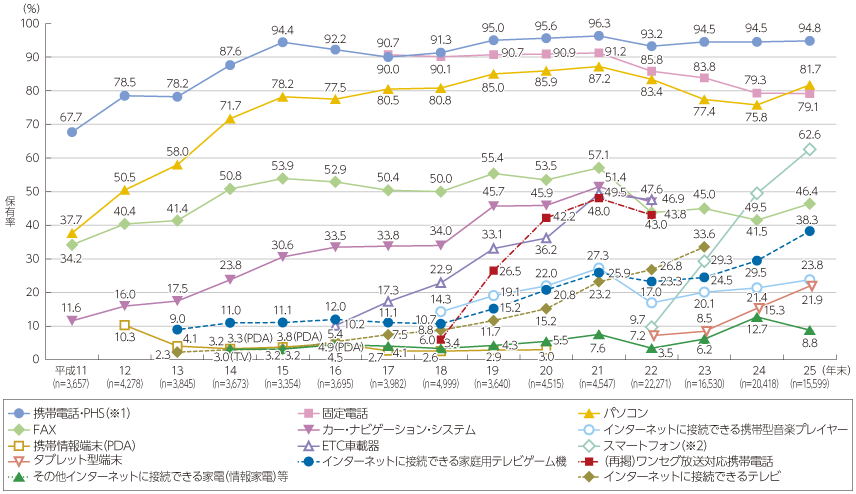
\includegraphics[width=160mm,bb=0 0 856 494]{images/mobiledevicespread.png}
    \caption{情報通信端末世帯保有率の推移(出典:\cite{communicationreport})}
    \label{fig:mobiledevicespread}
  \end{center}
\end{figure}
平成22年には9.7%しかなかったスマートフォンの普及率は、
平成25年には62.6%と急激に成長している。
平成22年から平成25年の3年間で52.9%の伸びを見せており、
これはパソコンの成長率が最も伸びた平成11年から平成14年の
伸び率を大きく上回る数字となっている。
このデータからもスマートフォンの普及は未だかつてないほどの
速度で進んでいることがわかる。

\subsection{モバイルデバイスの用途}

スマートフォンはパソコンの様に多くのことができるが、
使用用途はある程度限られているのが現状である。


現在、
これらのモバイルデバイスを使う上で日本語の入力は欠かすことができない操作である。
デバイスの性能は携帯電話の頃から劇的に向上している。
パソコンに遜色ないようなメモリやCPUを積んでいるものも多く市販されている。
しかし文字入力に関してはあまり成長していない。

文字入力にもデバイスに適したよりよいものがある。
文字入力のユーザの体験ももっと向上すべきである。
今回は日本人向けのシステムとして作った。

ユーザにはそれぞれコンテキストがある。
コンテキストによって入力したい単語は推測できるのではないか

\subsection{文字入力への機械増加}


\section{文字入力の歴史}


\section{問題点と期待}
楽天リサーチによる「スマートフォンに関する調査」
(出典:\cite{rakutensmartphone})によると、
スマートフォンを使うユーザーが挙げる不満点の中で
最も割合が大きいのが「文字入力がしにくい」ということである。
(出典:\cite{rakutensmartphone})
\begin{figure}
  \begin{center}
    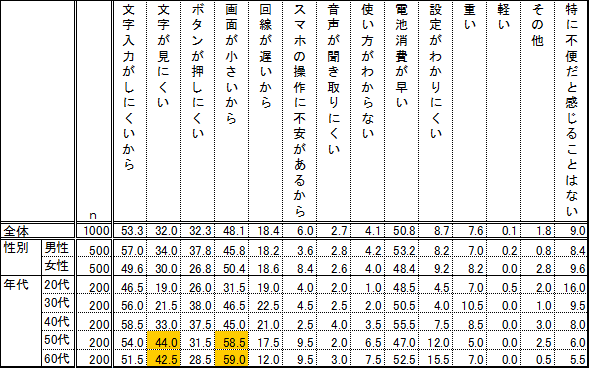
\includegraphics[width=140mm,bb=0 0 589 368]{images/dissatisfaction.png}
    \caption{スマートフォンを利用している際に不便だと感じる点(出典:\cite{rakutensmartphone})}
    \label{fig:dissatisfaction}
  \end{center}
\end{figure}

利用時間長すぎ
スマートウォッチやグーグルグラスなどでは文字入力めんどい
